\documentclass[12pt,UTF8,a4paper]{ctexart}
\usepackage[margin=2.5cm]{geometry}
\usepackage{graphicx}
\graphicspath{{figures/}}
\usepackage{booktabs}
\usepackage{amsmath}
\usepackage{caption}
\usepackage{hyperref}
\captionsetup{font=small}
\setlength{\parskip}{0.5em}

\title{\textbf{轻型螺旋桨验证机自主进近与着陆控制律}\\[0.5em]
\large SimplePlanes 2 飞行控制学习项目·SC-3 验证试验报告（封版版）}
\author{}
\date{2026 年 9 月 23 日}

\begin{document}
\maketitle
\thispagestyle{empty}

\begin{abstract}
本报告记录 SC-3 课题（TESTaircraft 轻型螺旋桨验证机全自动着陆）的控制律设计与试飞验证结果。在平台不提供跑道坐标接口的约束下，建立了以出生点自标定为基础的两状态着陆律：下滑段采用下沉率跟踪（方向无关），拉平段以迎角保持环经高度权重渐进接管，速度通道按油门/减速板包络分区管理，接地后以配平接力保持主轮承载。经十七轮迭代，末版实现 183 m 高度进入、约 1.8 km 沿跑道下滑、接地姿态 $+2.0^\circ$、接地下沉 2.8 m/s、主轮先触且前轮柔和跟随的全自主着陆。试验判定着陆主链路验收通过并封版；远距自动进近（SC-3b）完成可行性论证并列为下一课题。
\end{abstract}

\section{任务定义与被试平台}
被试平台为此前定型的 TESTaircraft：前三点起落架螺旋桨验证机。机体档案两项实测特性直接决定了着陆律的设计边界：其一，低速包线极宽（42 m/s 可控，零速不失速并可自改出），故经典能量保护逻辑（低速限制抬头、三档失速守卫）全部无需设置；其二，机体阻力大，下滑需主动能量管理而非纯滑翔。

平台约束方面，经对游戏运行时的系统检索确认：不存在任何可被机载脚本查询的跑道世界坐标接口（相关枚举与组件均为装饰性或无消费者），因此机场基准采用\textbf{出生点自标定}方案——起飞滑跑帧（近地判据成立）自动记录当前位置、航向与地面标高作为跑道基准，与"出生即位于跑道中线"的世界规则一致。

\section{控制律架构（定版 v4.17）}
模式由 MFD 按钮 9 切换，仅两状态：下滑（GLIDE）与滑跑（ROLLOUT）。全部外环位于 Lua（真时间步长），舵面内环沿用机体表达式侧已验证结构。

\subsection{横向通道}
在跑道坐标系下分解纵向投影 $s$ 与右偏距 $l$，目标航向取 $\psi_{tgt} = \psi_{rwy} - 0.02^\circ/\mathrm{m}\cdot l$，滚转杆量按航向偏差比例（增益 0.010，限幅 $\pm0.45$）。该形式对"到跑道点距离"奇异免疫。

\subsection{垂直通道：两段式权重交接}
下滑段跟踪下沉率指令 $\dot h_{cmd} = -V_G \tan 3.5^\circ$（比例增益 2.2，含坡度补偿），替代早期"标高目标线"方案——后者在越过基准点反向飞行时构成发散目标，曾使姿态环长期饱和。拉平窗（AGL 45 m 至 15 m）内权重 $w_a$ 线性升至 1，指令由下沉率环渐进交予迎角保持环：
\[
\theta_{cmd} = (1-w_a)\,\theta_{path} + w_a\big[K_\alpha(\alpha^\ast - \alpha) + K_i\,\Sigma_{w}(\alpha^\ast-\alpha) + \text{坡度补偿}\big],
\]
其中 $\alpha^\ast = 8^\circ$，$\Sigma_{w}$ 为拉平窗内累积的积分项（进窗才累积、出窗清零、限幅 $\pm10^\circ$；积分速率 $1.2\ ^\circ/\mathrm{s}$——拉平窗全长约 4 s，慢速率积分无法建立所需舵偏）。积分项的引入源于纯比例环的静差：实测同一舵偏下迎角平台约 5.2$^\circ$，无法逼近接地姿态要求。

\subsection{速度通道：执行器包络分区}
油门与减速板按空速轴分区，禁止互搏：加油门仅允许于低速侧（$V<51$ m/s，或"能量债"且 $V<55$），收油门于 $V>58$，减速板 $V>56$ 缓开（1/s）、$V\ge64$ 全开、低速侧强制快收（4/s）。其中"能量债"判据定义为实际下沉超过指令 1 m/s 以上——该判据早期版本曾同时豁免油门与刹车，在大阻力机上恒真，构成超速保护伞，已裁撤为仅作用于低速侧。减速板的机体侧前提是将螺旋桨顺桨机构从刹车轴解耦（同轴多零件隐性联动，见 §4）。

\subsection{接地与滑跑}
近地判据 AGL $<4$ m（考虑高度传感器地面读数下限 1.6--2.0 m，阈值必须高于测量地板）触发：油门归零、刹车轴满输入（轮刹+减速板全开）、油门带解除；俯仰通道不即时交还，保持最后杆位 1.5 s 后释放，并在释放同一时刻施加机头上仰配平 $-0.2$（约 20\%）持续压尾，使主轮保持承载、前轮在减速中柔和加载。空速低于 5 m/s 或 40 s 超时后全通道交还。

\section{平台级发现与方法论要点}
\begin{itemize}
\item \textbf{迎角符号反约定}：脚本侧迎角读数实为 $\gamma-\theta$，与空气动力学约定符号相反。定罪方法为三方几何核算（俯仰角、由下沉/地速反算的航迹角、读数迎角）。据此确立规程：任何新传感器量建律前先做独立几何核算定符号。
\item \textbf{轴到舵面的映射系数墙}：机体出厂升降舵律使满杆仅对应半舵偏转，53 m/s 下顶格迎角 5.2$^\circ$；将表达式增益翻倍以解锁满舵权限，同时按比例减半脚本侧姿态环增益以保持环路总增益——跨侧耦合参数改任何一侧必须审计另一侧。
\item \textbf{执行器隐性联动}：刹车轴同时绑定轮刹、螺旋桨刹车与减速板，空中使用等价于切断拉力，导致能量崩盘与俯仰失控的复合故障。据此确立：控制律设计前按轴枚举全部绑定零件，双向轴逐场景核每个零件的后果。
\item \textbf{判读尺修正}：着陆滑跑中刹车减速度（约 1.2 g）产生显著低头力矩，滑跑段俯仰姿态不具备拉平质量判读价值；全部姿态类指标只取接地前窗口。
\item \textbf{验收指标的性质审查}：$\alpha\ge6^\circ$ 一类中间量指标在航迹收敛后自然回落（$\alpha = \theta - \gamma$），应以结果量（接地姿态、下沉率、主轮先触）为最终判据。
\end{itemize}

\section{试验结果}
表~\ref{tab:score} 给出关键迭代轮次的接地窗口指标（均为接地前判读）。自 v4.10 起主轮先触稳定达成，v4.17 在接地姿态与下沉率两项实现质变，前轮触地间隔内姿态保持正仰角，全程无弹跳、无需人工接管。

\begin{table}[h]\centering\small
\setlength{\tabcolsep}{5pt}
\caption{接地窗口指标演进（判读尺：接地前）}
\begin{tabular}{lcccl}
\toprule
版本 & 速度 (m/s) & 俯仰 ($^\circ$) & 下沉 (m/s) & 主轮先触 \\
\midrule
v4（初版） & 55 & $-1.5$ & $\approx 6.7$ & 否（前轮拍地） \\
v4.10 & 61 & $+2.4$ & $\approx 5.0$ & 是（前轮 1.1 s） \\
v4.16 & 54 & $+0.1$ & $4.7$ & 是（前轮 0.6 s） \\
\textbf{v4.17（封版）} & \textbf{56} & \textbf{$+2.0$} & \textbf{2.8} & \textbf{是（前轮 $\sim$0.3 s）} \\
\bottomrule
\end{tabular}\label{tab:score}
\end{table}

封版版实测全程（日志实例 60268）：183 m 高度进入，沿跑道中线下滑约 1.79 km，接地后 4.5 s 内减速至停止，横向偏距不大于 5 m，航向偏差收敛于 $\pm1.2^\circ$ 内；图~\ref{fig:landing} 给出剖面、能量、横向与接地窗姿态/迎角四通道记录。

\begin{figure}[h]\centering
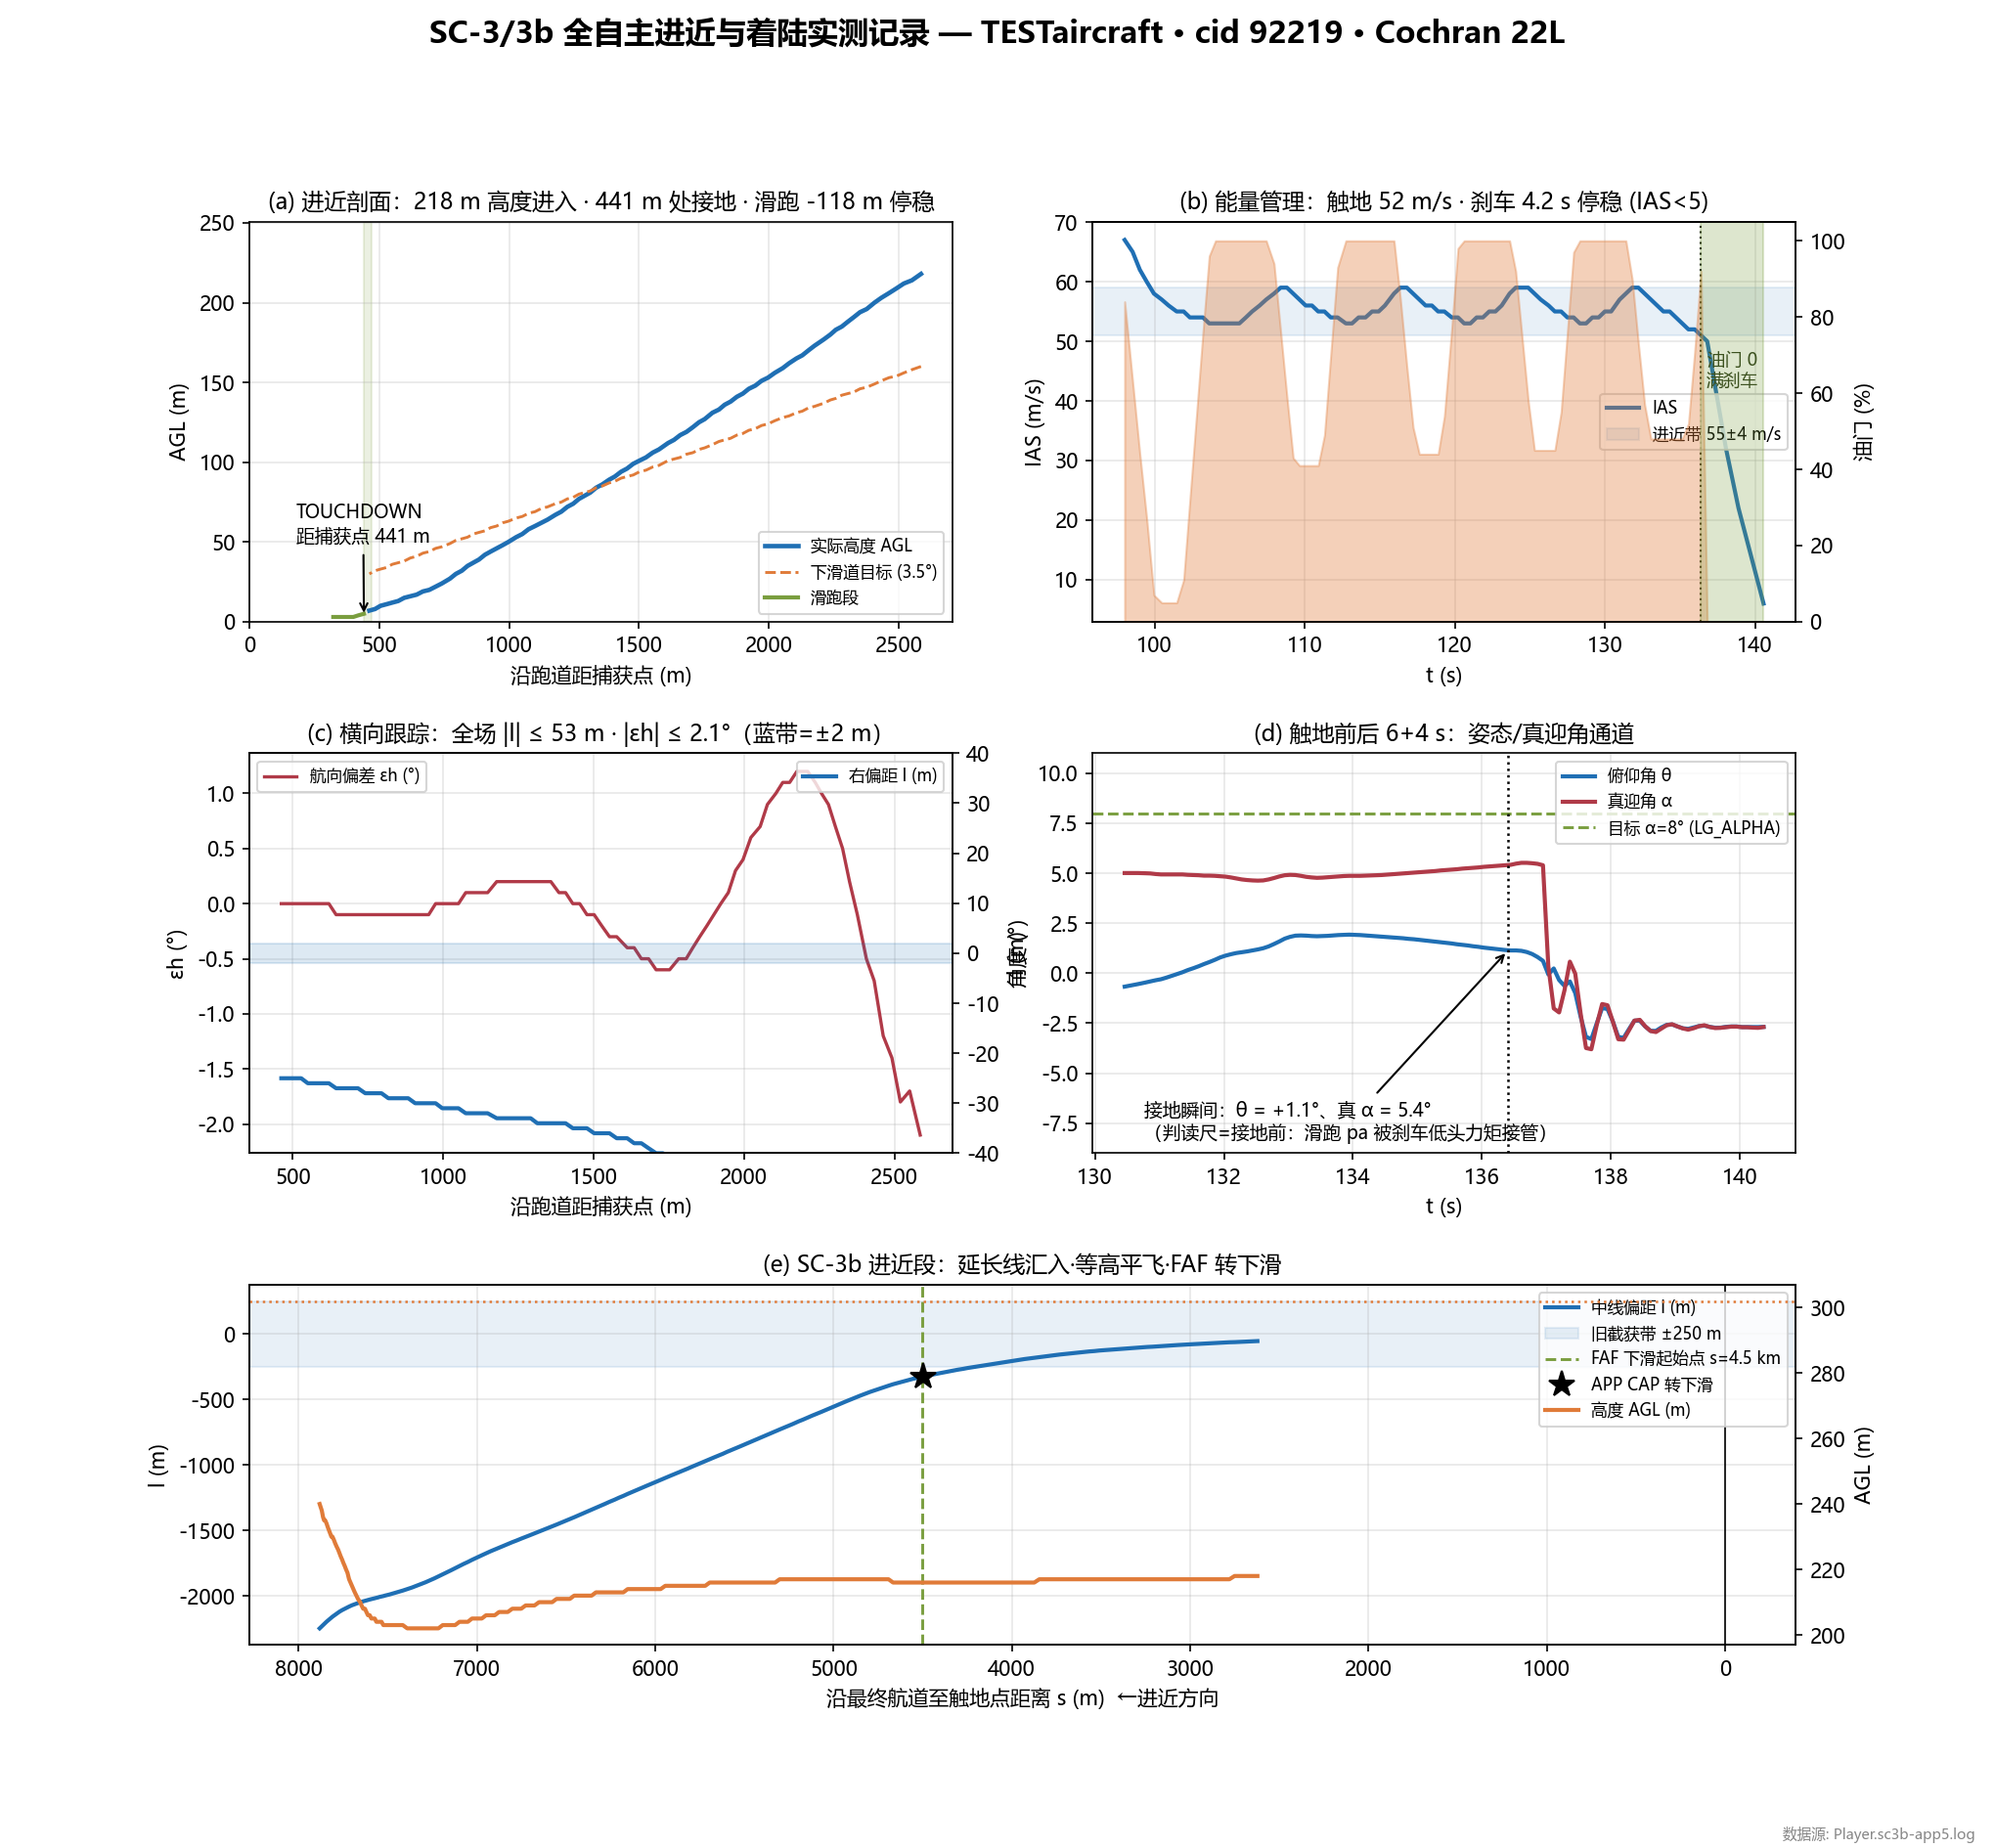
\includegraphics[width=0.98\textwidth]{sc3-landing-report.png}
\caption{SC-3 全自主着陆实测记录（v4.17）：(a) 进近剖面；(b) 速度与油门/刹车管理；(c) 横向跟踪；(d) 触地前后 6+4 s 姿态与真迎角通道。}
\label{fig:landing}
\end{figure}

\section{遗留项与展望}
已记录不修复项：速度通道存在幅值约 $\pm4$ m/s、周期约 7 s 的极限环（油门带与阻力耦合），经多局验证对着陆品质无影响。后续课题 SC-3b（远距自动进近）已完成可行性论证：全地图跑道头坐标、磁差与标高可从游戏资源包的静态出生点表完整提取（四机场七跑道，含对头配对编号），与运行时自标定数据互证了坐标映射，规划层仅需在现有两状态律前端增加"选跑道—建立入口—截获"几何链，无新增平台依赖。

\section{结论}
SC-3 着陆主链路（对准—下滑—拉平—接地—滑跑—交还）在无任何人工接管条件下闭环达成，控制律定版 v4.17 并封版。本课题沉淀的符号核算、映射审计、包络分区与判读尺四类方法与此前课题合并，构成该平台飞控工程的完整作业规范。

\end{document}
